\providecommand{\curso}{Séptimo Básico}
\providecommand{\colegio}{Colegio Divina Pastora}
\providecommand{\tituloDocumento}{Prueba}
\providecommand{\subtituloDocumento}{Sintesis y descripción de datos}
\providecommand{\tituloItem}{Pregunta }

\documentclass{cdplf-prueba}


\begin{document}

\begin{tcbraster}[enhanced,raster columns=3,raster width=\linewidth,raster column skip=3pt,raster force size=false]
    \begin{caja}[title={\sffamily\scshape\bfseries Nombre},height=30pt,add to width=4cm]
    \end{caja}
    \begin{caja}[title={\sffamily\scshape\bfseries Puntaje},height=30pt,add to width=-2cm]
    \end{caja}
    \begin{caja}[title={\sffamily\scshape\bfseries Nota},height=30pt,add to width=-2cm]
    \end{caja}                    
\end{tcbraster}

\subsection*{Objetivos de la evaluación}
\begin{itemize}[]
    \item Sintetizar datos mediante una tabla de frecuencias.
    \item Representar datos mediante un gráfico de barras.
    \item Determinar medidas de tendencia central para un grupo de datos.
    \item Explicar y fundamentar soluciones propias y los procedimientos utilizados.
\end{itemize}

\subsection*{Instrucciones generales}

La evaluación está diseñada para realizarse dentro de la clase en 60 minutos, es individual y 
con nota al libro. Además, si usted lo considera necesario, puede usar calculadora para su
desarrollo.

Por otro lado, cualquier acto de deshonestidad durante la evaluación, será sancionado según 
el reglamento del colegio.

\subsection*{Pauta de cotejo}

En la corrección de la evaluación, se asignará puntaje a cada respuesta según
los criterios que se encuentran detallados en la tabla a continuación.

\begin{center}
    \begin{tblr}{width=\linewidth,colspec={X[1,c]|X[6]}, hline{1,Z} = {1}{-}{}, hline{1,Z} = {2}{-}{}, 
        hlines, cells={valign=m}, row{1} = {bg=black!15}}
        Puntaje asignado & \SetCell{c} Criterios o indicadores \\
        +50\% & Señala clara y correctamente cuál es la solución o el resultado de la pregunta hecha
        en el enunciado. \\ 
        +50\% & Incluye un desarrollo que relata de manera clara y ordenada los procedimientos 
         \mbox{necesarios} para solucionar la problemática. En caso de estar incompleto o con 
         \mbox{errores} el desarrollo, se asignará puntaje parcial si se muestra dominio de los 
         con\-tenidos y conceptos involucrados. \\
        0\% &  La respuesta es incorrecta. De haber desarrollo, este tiene errores conceptuales.\\
    \end{tblr}    
\end{center}

\vspace*{\fill}
\begin{center}
    \begin{tikzpicture}[ampersand replacement=\&,]
        %\node (A) [opacity=0.4] {\includegraphics[width=2cm]{../flork3.jpg}};
        \node (B) [font=\slshape,text width=12cm]
        {``Cree en ti mismo y en lo que eres. Sé consciente de que hay algo en tu interior %
        que es más grande que cualquier obstáculo''};
        \node [left=0mm of B,opacity=0.4] {\pgfornament[width=2cm]{37}};
        \node [right=0mm of B,opacity=0.4] {\pgfornament[width=2cm]{38}};
    \end{tikzpicture}
\end{center}
\vspace*{\fill}
\newpage

%\parte 
\begin{tcolorbox}[boxrule=1pt,colback=white,leftrule=3mm]
    \raggedright Resuelva los problemas que se encuentran a continuación. Para esto, no olvide 
    incluir un desarrollo pertinente y la respuesta al enunciado en los espacios señalizados.        
\end{tcolorbox}
 
%\pregunta 
\subsection{} Complete la siguiente tabla de frecuencias con los datos entregados a continuación [4 puntos].
\\[3pt]
\underline{Datos}: 12 {\textbullet} 4 {\textbullet} 9 {\textbullet} 14 {\textbullet} 5 {\textbullet} 12 {\textbullet} 12 {\textbullet} 9 {\textbullet} 12 {\textbullet} 14 {\textbullet} 6 {\textbullet} 12 {\textbullet} 1 {\textbullet} 10 {\textbullet} 13 {\textbullet} 6 {\textbullet} 12 {\textbullet} 8 {\textbullet} 12 {\textbullet} 8 {\textbullet} 11 {\textbullet} 12 {\textbullet} 9 {\textbullet} 13 {\textbullet} 11 {\textbullet} 7 {\textbullet} 13 {\textbullet} 9 {\textbullet} 10 {\textbullet} 6 {\textbullet} 10 {\textbullet} 13 {\textbullet} 13 {\textbullet} 13 {\textbullet} 12 {\textbullet} 9 {\textbullet} 2 {\textbullet} 15 {\textbullet} 11 {\textbullet} 7
\vspace{3pt}

% 1 	&	      1 	&	 0.025 	&	      1 	&	 0.025 \\
% 2 	&	      1 	&	 0.025 	&	      2 	&	 0.050 \\
% 4 	&	      1 	&	 0.025 	&	      3 	&	 0.075 \\
% 5 	&	      1 	&	 0.025 	&	      4 	&	 0.100 \\
% 6 	&	      3 	&	 0.075 	&	      7 	&	 0.175 \\
% 7 	&	      2 	&	 0.050 	&	      9 	&	 0.225 \\
% 8 	&	      2 	&	 0.050 	&	     11 	&	 0.275 \\
% 9 	&	      5 	&	 0.125 	&	     16 	&	 0.400 \\
% 10 	&	      3 	&	 0.075 	&	     19 	&	 0.475 \\
% 11 	&	      3 	&	 0.075 	&	     22 	&	 0.550 \\
% 12 	&	      9 	&	 0.225 	&	     31 	&	 0.775 \\
% 13 	&	      6 	&	 0.150 	&	     37 	&	 0.925 \\
% 14 	&	      2 	&	 0.050 	&	     39 	&	 0.975 \\
% 15 	&	      1 	&	 0.025 	&	     40 	&	 1.000 \\
\begin{center}
    \begin{tblr}{width=0.8\linewidth,colspec={X[1,c]X[3,c]X[3,c]X[3,c]X[3,c]},hlines,vlines,hline{2,Z} = {1}{-}{},hline{2,Z} = {2}{-}{},row{even}={black!10},
        row{1}={font=},rowsep=5pt,cells={valign=m}}
                &Frecuencia & Probabilidad  & Frecuencia Acumulada & Probabilidad Acumulada \\
                1 & & & & \\
                2 & & & & \\
                4 & & & & \\
                5 & & & & \\
                6 & & & & \\
                7 & & & & \\
                8 & & & & \\
                9 & & & & \\
                10 & & & & \\
                11 & & & & \\
                12 & & & & \\
                13 & & & & \\
                14 & & & & \\
                15 & & & & \\
    \end{tblr}
    \end{center}

 \subsection{} Represente los siguientes datos en un gráfico de barras [2 puntos].
%  3 	&	      1 	&	 0.025 	&	      1 	&	 0.025 \\
%  4 	&	      1 	&	 0.025 	&	      2 	&	 0.050 \\
%  7 	&	      3 	&	 0.075 	&	      5 	&	 0.125 \\
%  8 	&	      8 	&	 0.200 	&	     13 	&	 0.325 \\
%  9 	&	      7 	&	 0.175 	&	     20 	&	 0.500 \\
% 10 	&	      5 	&	 0.125 	&	     25 	&	 0.625 \\
% 11 	&	      5 	&	 0.125 	&	     30 	&	 0.750 \\
% 12 	&	      6 	&	 0.150 	&	     36 	&	 0.900 \\
% 13 	&	      1 	&	 0.025 	&	     37 	&	 0.925 \\
% 14 	&	      2 	&	 0.050 	&	     39 	&	 0.975 \\
% 16 	&	      1 	&	 0.025 	&	     40 	&	 1.000 \\
%
\begin{tcolorbox}[blanker,sidebyside,lefthand width=0.26\linewidth,box align=top,halign upper=center]
    \begin{center}
    \begin{tblr}{width=0.8\linewidth,colspec={X[3,c]X[9,c]},hlines,vlines,hline{2,Z} = {1}{-}{},hline{2,Z} = {2}{-}{},row{even}={black!10},
        row{1}={font=},rowsep=3pt,cells={valign=m}}
                    & Frecuencia     \\
                3 	&	      1 	 \\
                4 	&	      1 	 \\
                7 	&	      3 	 \\
                8 	&	      8 	 \\
                9 	&	      7 	 \\
                10 	&	      5 	 \\
                11 	&	      5 	 \\
                12 	&	      6 	 \\
                13 	&	      1 	 \\
                14 	&	      2 	 \\
                16 	&	      1 	 \\
    \end{tblr}
    \end{center}
    %
    \tcblower
    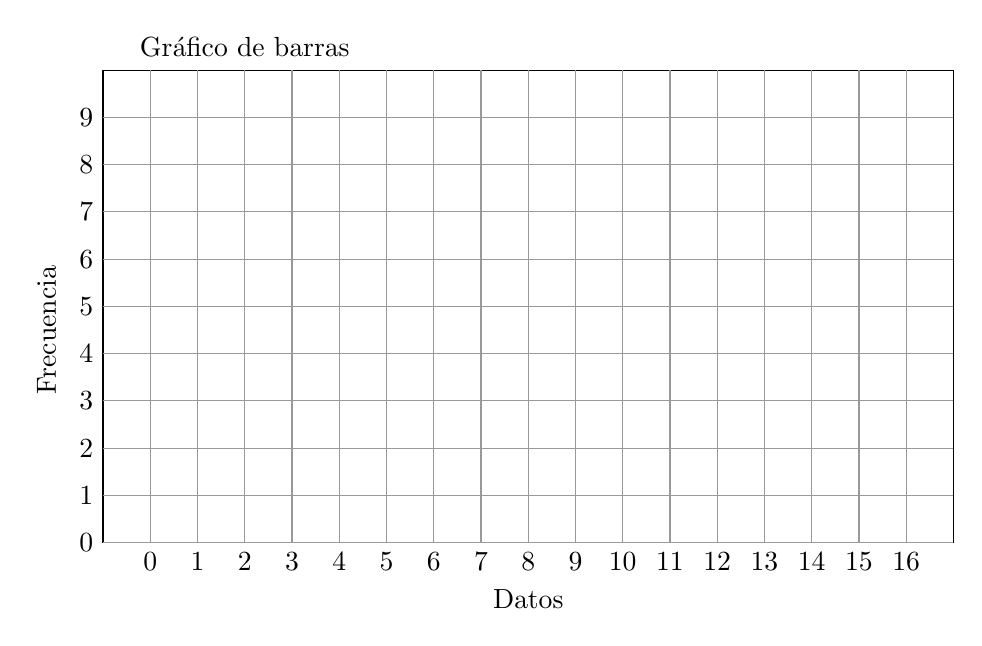
\begin{tikzpicture}[ampersand replacement=\&,y=0.6cm,x=0.6cm]
        \draw (-1,0) rectangle (17,10);
        \foreach \x in {0,1,...,16} {
            \draw [draw=black!40] (\x, 10) -- (\x, 0) node[below] {$\x$};
        }
        \foreach \y in {0,1,...,9} {
            \draw [draw=black!40] (17,\y) -- (-1,\y) node [left] {$\y$};
        }
        \node at (8,-1.2) {Datos};
        \node at (-2.2,4.5) [rotate=90] {Frecuencia};
        \node at (2, 10.5) [font=] {Gráfico de barras};
    \end{tikzpicture}
\end{tcolorbox}

\def\respuestas{%
\begin{tcbraster}[enhanced,raster columns=4,raster width=1\linewidth,raster column skip=20pt]
    \begin{caja}[title={\sffamily\scshape\bfseries Moda},height=30pt]
    \end{caja}
    \begin{caja}[title={\sffamily\scshape\bfseries Media},height=30pt]
    \end{caja}
    \begin{caja}[title={\sffamily\scshape\bfseries Mediana},height=30pt]
    \end{caja}  
    \begin{caja}[title={\sffamily\scshape\bfseries Rango},height=30pt]
    \end{caja}                    
\end{tcbraster}}

\subsection{} Para cada grupo de datos, determine las medidas pedidas [1 punto por cada medida]. 

\begin{tasks}[label={\tcbox[colback=black!60, colframe=black!60, coltext=white, on line, boxsep=0pt, left=3pt, right=3pt, top=2pt, bottom=2pt]{\sffamily\bfseries\Alph*}},
item-indent=1.2cm,column-sep=20pt,label-offset=0.3cm,label-width=15pt,after-item-skip=10pt]
    \task! \underline{Datos:} 6 {\textbullet} 8 {\textbullet} 11 {\textbullet} 6 {\textbullet} 11 {\textbullet} 10 {\textbullet} 11 {\textbullet} 12 {\textbullet} 8 {\textbullet} 13 {\textbullet} 8 {\textbullet} 11 {\textbullet} 7 {\textbullet} 9
    \vspace{10pt}\begin{desarrollo}[height=1.5cm]\end{desarrollo}\vspace{10pt}
    \respuestas
    \task! \underline{Datos:} 10 {\textbullet} 9 {\textbullet} 8 {\textbullet} 9 {\textbullet} 15 {\textbullet} 7 {\textbullet} 8 {\textbullet} 7 {\textbullet} 13 {\textbullet} 11 {\textbullet} 9 {\textbullet} 13 {\textbullet} 13 {\textbullet} 13 {\textbullet} 16
    \vspace{10pt}\begin{desarrollo}[height=1.5cm]\end{desarrollo}\vspace{10pt}
    \respuestas
\end{tasks}


\end{document}